%-----------------------------------------------------------------------------------------------%
%
% Maret 2019
% Template Latex untuk Tugas Akhir Program Studi Sistem informasi ini
% dikembangkan oleh Inggih Permana (inggihjava@gmail.com)
%
% Template ini dikembangkan dari template yang dibuat oleh Andreas Febrian (Fasilkom UI 2003).
%
% Orang yang cerdas adalah orang yang paling banyak mengingat kematian.
%
%-----------------------------------------------------------------------------------------------%


%-----------------------------------------------------------------------------%
\chapter{\babTiga}
%-----------------------------------------------------------------------------%
Kerangka penelitian ini adalah langkah demi langkah dalam penyusunan Tugas Akhir mulai dari Tahap Perencanaan penelitian hingga Tahap Hasil dan Dokumentasi. Berikut ini adalah gambar Metodologi Penelitian dapat dilihat pada Gambar 3.1.
\begin{figure}
	\centering
	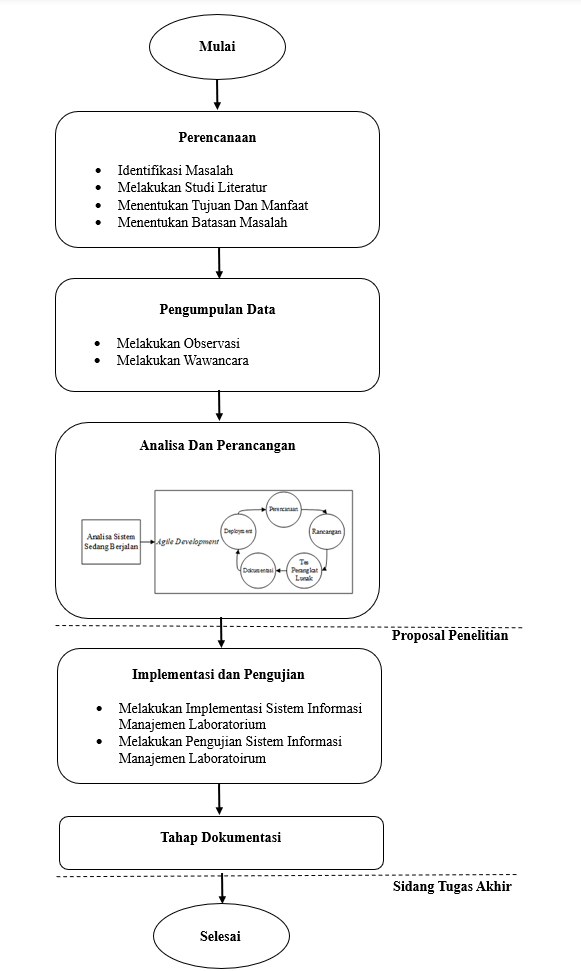
\includegraphics[width=0.92\linewidth]{konten//gambar/metodologi-penelitian.png}
	\caption{Metodologi Penelitian}
	\label{fig:enter-label}
\end{figure}
%-----------------------------------------------------------------------------%

\section{Tahap Perencanaan}
Langkah pertama dalam penelitian ini adalah mengidentifikasi masalah, studi literatur, menentukan tujuan dan manfaat, menentukan batasan masalah, menentukan data-data serta informasi yang dibutuhkan saat penelitian.

\subsection{Identifikasi Masalah}
Pada tahap ini, tujuan dari penelitian ini adalah untuk mengembangkan SITARIS SI menjadi sistem manajemen laboratorium. Dari masalah yang telah ditemukan dan disebutkan sebelumnya, rumusan masalah yang dihasilkan dari penelitian ini adalah “Bagaimana menerapkan metode Agile dalam pengembangan lebih lanjut SITARIS SI menjadi sistem manajemen laboratorium untuk meningkatkan kualitas, dan fungsionalitas sistem”.

\subsubsection{Observasi}
Pada tahap awal, peneliti melakukan pengamatan langsung pada studi kasus yang telah dipilih untuk mengidentifikasi kegiatan atau masalah yang terjadi pada studi kasus tersebut dan mengumpulkan data terkait.

\subsubsection{Wawancara}
Wawancara merupakan teknik pengumpulan data yang dilakukan melalui tatap muka dan tanya jawab langsung antara peneliti dan narasumber. Wawancara dilakukan untuk mendapatkan informasi secara tepat dan akurat dari narasumber yang terpercaya. Narasumber yang terkait pada penelitian ini yaitu bapak Tengku Khairil Ahsyar S.Kom., M.Kom., selaku Kepala Laboratorium Sistem Informasi.

\subsection{Studi Literatur}
Pada tahap ini, hal pertama yang dilakukan adalah melakukan penelitian literatur untuk mendapatkan informasi yang diperlukan untuk menulis tentang topik yang diangkat. Selain itu, kegiatan penelitian ini juga membantu mengetahui teori-teori, serta metode dan teknik yang berkaitan dengan topik atau masalah yang akan digunakan untuk mencapai tujuan yang diinginkan. Teori yang digunakan di sini berasal dari artikel jurnal.

\subsection{Menentukan Tujuan dan Manfaat}
Pada tahap ini, akan dibahas tentang rumusan kalimat yang menunjukkan adanya hasil, tujuan penelitian, dan apa yang diperoleh setelah penelitian selesai.

\subsection{Menentukan Batasan Masalah}
Pada tahap ini, yang dilakukan adalah membatasi subjek penelitian. Untuk mengumpulkan masalah, penelitian ini menggunakan observasi dan wawancara serta penelitian ini menggunakan metode Agile Development.

\section{Tahap Analisis dan Perancangan}
Langkah ketiga dalam penelitian ini adalah menganalisis sistem yang sedang berjalan yaitu SITARIS SI.

\subsection{Menganalisis SITARIS SI}
Analisis SITARIS SI merupakan tahap krusial dalam pengembangan sistem. Proses ini melibatkan pemeriksaan menyeluruh terhadap berbagai aspek sistem untuk memastikan kualitas dan efektivitasnya. Langkah pertama dalam pengembangan ini adalah evaluasi fungsionalitas sistem. Peneliti akan memeriksa setiap fitur SITARIS SI untuk memastikan bahwa semua berfungsi sesuai dengan spesifikasi yang telah ditentukan. Ini mencakup pengujian setiap modul, menu, dan fungsi dalam sistem untuk memverifikasi bahwa mereka beroperasi dengan benar dan memberikan output yang diharapkan.

\subsection{Agile Development}
Agile Development (Analisa Sistem Usulan) Berikut adalah penjelasan mengenai tahapan metode Agile.
\begin{enumerate}
	\item Tahap Perencanaan dimana pihak pengembang sistem dan klien, Laboratorium Prodi Sistem Informasi, dapat melakukan perencanaan kebutuhan yang akan dikerjakan.
	\item Tahap Rancangan dimana pihak pengembang sistem dapat merancang alur dan sistem manajemen yang akan dibuat.
	\item Tahap Pengujian perangkat lunak dimana pihak pengembang sistem telah membuat sistem dan melakukan pengecekan apakah ada kesalahan dari sistem yang telah dibuat, dan jika ada kesalahan maka harus diperbaiki.
	\item Tahap Dokumentasi dimana memberikan kemudahan bagi pengguna untuk memelihara sistem kedepannya.
	\item Tahap Implementasi dimana pengembang sistem dapat menjamin kualitas sistem yang telah dibuat dengan menguji kualitas, keamanan, dan kecepatan dari sistem yang telah dibuat.
\end{enumerate}

\section{Tahap Implementasi dan Pengujian}
Selanjutnya melakukan tahap implementasi dan pengujian pada sistem. Langkah-langkahnya adalah sebagai berikut:
\begin{enumerate}
	\item Implementasi Dalam penelitian ini bahasa pemrograman yang dipilih untuk membangun sistem adalah PHP dengan framework CodeIgniter4 dan VS Code sebagai editor codingnya.
	\item Pengujian Sistem Setelah sistem selesai dibangun dengan menggunakan bahasa pemrograman yang dipilih, langkah selanjutnya adalah menguji sistem tersebut agar mengetahui suatu kesalahan yang terjadi. Pengujian dilakukan dengan menggunakan Black Box Testing dan Manual Testing.
\end{enumerate}

\section{Tahap Dokumentasi}
Langkah terakhir ialah melakukan dokumentasi semua kegiatan yang telah dilakukan mulai dari awal hingga akhir dengan membuat laporan Tugas Akhir.